\documentclass[12pt, twoside]{report}

% Paquetes LaTeX y estilos globales
\usepackage[utf8]{inputenc}
% \usepackage{subfigure}
\usepackage{caption}
\usepackage{subcaption}
\usepackage{multicol}
\usepackage{xcolor}
\usepackage[spanish,es-tabla]{babel}
\usepackage[utf8]{inputenc}
\usepackage{graphicx}
\usepackage{titlesec}
\usepackage[bookmarks,breaklinks,colorlinks=true,allcolors=blue]{hyperref}
\usepackage{listings}
\usepackage{inconsolata}
\usepackage{float}
\usepackage{comment}

% \usepackage[square,numbers]{natbib}
\usepackage{natbib}
\usepackage[nottoc]{tocbibind}

%\AtBeginDocument{
%  \renewcommand{\bibsection}{\chapter{\bibname}}
%} % Bibliografia en capitulo numerado

\usepackage{geometry}
\usepackage{amsmath}
\usepackage{parskip}
\usepackage[official]{eurosym}
\usepackage{todonotes}
\usepackage{csquotes}

\usepackage{lipsum}
\usepackage{multirow}

\usepackage[es]{datetime2}
\DTMlangsetup{showdayofmonth=false}

\selectlanguage{spanish}

%Gestión de anexos
\usepackage{appendix}
\renewcommand{\appendixname}{Anexos}
\renewcommand{\appendixtocname}{Anexos}
\renewcommand{\appendixpagename}{Anexos}
% Formato del título de capítulos y secciones
% \titleformat{\chapter}[block]{\titlerule[0.8pt]\normalfont\huge\bfseries}{\thechapter.}{.5em}{\Huge}[{\titlerule[0.8pt]}]
% \titlespacing*{\chapter}{0pt}{-19pt}{25pt}
% \titleformat{\section}[block]{\normalfont\Large\bfseries}{\thesection.}{.5em}{\Large}

\titleformat{\chapter}[block]{\normalfont\huge\bfseries}{\thechapter.}{.5em}{\Huge}[{\titlerule[0.8pt]}]
\titlespacing*{\chapter}{0pt}{-19pt}{25pt}
\titleformat{\section}[block]{\normalfont\Large\bfseries}{\thesection.}{.5em}{\Large}

% Formato del código fuente con lstlisting
\lstset{
  basicstyle=\ttfamily,
  breaklines=true,
}

% Márgenes
\geometry{
    a4paper,
    margin=2.75cm
}

% Limite de profundidad del índice
\setcounter{tocdepth}{2}

% Indentación de párrafos
\setlength{\parindent}{1cm}

\renewcommand{\lstlistingname}{Extracto de código}
\renewcommand*{\lstlistlistingname}{Índice de extractos de código}

%------------ Caption debajo de las tablas --------------%
\DeclareCaptionLabelSeparator*{spaced}{\\[1.5ex]}
\captionsetup[table]{textfont=it,format=plain,justification=justified,
  singlelinecheck=false,labelsep=spaced,skip=0pt}

\lstset{
  basicstyle=\ttfamily,
  columns=fullflexible,
  frame=none,
  breaklines=true,
  postbreak=\mbox{},
  xleftmargin=.4\textwidth, 
  xrightmargin=.2\textwidth
} 
\usepackage{caption}
\usepackage{subcaption}
\usepackage{graphicx}
\DeclareCaptionFormat{custom}
{%
    \textbf{#1#2}\textit{\small #3}
}
\captionsetup{format=custom}

% Con \hypersetup podremos introducir los metadatos para la descripción del documento PDF. Recuerda modificarlo cuando transformes el documento.
\hypersetup{ 
    pdfauthor={Javier Arambarri Calvo}
    pdftitle={[OP_Pr2_Flexsim]}
    pdfsubject={Organización de la Producción}
    pdfkeywords{Palabras clave del documento}
    pdflang={Español}
    pdfcreator={Overleaf}
}

% Comienzo del documento
\begin{document}

    % FRONTMATTER: portadas y secciones no numeradas
    
\begin{center}

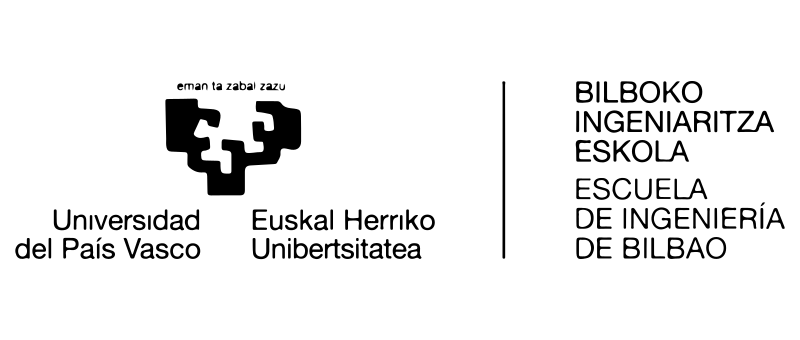
\includegraphics[width=0.65\textwidth]{source/images/logoEIB.png} 




\vspace*{2cm}
\begin{Large}
SISTEMAS DE GESTIÓN DE SEGURIDAD DE SISTEMAS DE INFORMACIÓN
\end{Large}

\vspace*{1cm}
\begin{Large}
GRADO EN INGENIERÍA INFORMÁTICA DE GESTIÓN Y SISTEMAS DE INFORMACIÓN
\end{Large}

\vspace*{2.5cm}

\textbf{\huge Euskoróscopo:\\ cómo usar el sistema web}\\
\vspace{1cm}
\textbf{\huge Entrega 1}% Aquí el título de su trabajo 
% Si el título del trabajo supera un párrafo añadir el comando \bigskip antes del título para que no se solapen dichos párrafos


\vspace*{1.5cm}

{\Large Adair Gondan Alonso\\Sergio Lusa Coria\\Javier Arambarri Calvo} % Aquí su nombre



\vspace*{1.5cm}

Bilbao, 14 de octubre de 2023\\


\end{center}

\thispagestyle{empty} % Impide que se incluya número de página en la portada

\clearpage\setcounter{page}{-1} % Comienza a incluir números de página a partir de aquí
\pagenumbering{arabic} % En números romanos  

\chapter*{Notas}
%\input{source/content/abstract}
\noindent Guía acerca de cómo usar el sistema web desarrollado. Este trabajo corresponde a la asignatura de Sistemas de Gestión de Seguridad de Sistemas de Información, cursada en el tercer año del grado en Ingeniería Informática de Gestión y Sistemas de Información.\\
\newline
En esta primera entrega se ha implementado un sistema web de temática libre, en nuestro caso una web de horóscopos llamada \textbf{Euskoróscopo}, utilizando HTML, PHP, CSS y JavaScript. No se ha tratado el tema de la seguridad en esta entrega, puesto que el objetivo es realizar el sistema lo más inseguro posible con el fin de buscar, actualizar y corregir las vulnerabilidades en la siguiente entrega.\\
\newline
El sistema puede encontrarse en el siguiente repositorio:\\
\href{https://github.com/Adair-GA/Seguridad_Web/tree/entrega_1}{https://github.com/Adair-GA/Seguridad\_Web/tree/entrega\_1}
\newline

\chapter{Funcionamiento del sistema}
\section{Arranque o acceso y página principal}
Accedemos al sistema web mediante su dirección url o desplegando el sistema mediante Docker.\\ En nuestro caso, tendremos que desplegar el sistema mediante Docker.
\newline
Si estamos desplegando el sistema por primera vez en el dispositivo o la base de datos ha sido modificada desde el último arranque, tendremos que importar la base de datos actualizada. Es necesario tener el sistema arrancado. Todo ello está descrito en el README.md\\

\begin{comment}
\begin{lstlisting}
$ docker-compose up -d
\end{lstlisting}

Para ello, accederemos a \textit{phpMyAdmin} desde \hyperlink{http://localhost:8890/}{http://localhost:8890/} en el navegador, e iniciamos sesión como administrador:
\begin{itemize}
    \item Usuario: \textbf{admin}
    \item Contraseña: \textbf{test}
\end{itemize}
La configuración del usuario y contraseña administrado de la base de datos se indica durante la creación de la imagen de MariaDB en el archivo \textit{docker-compose.yml}.
\begin{figure}[h]
\begin{center}
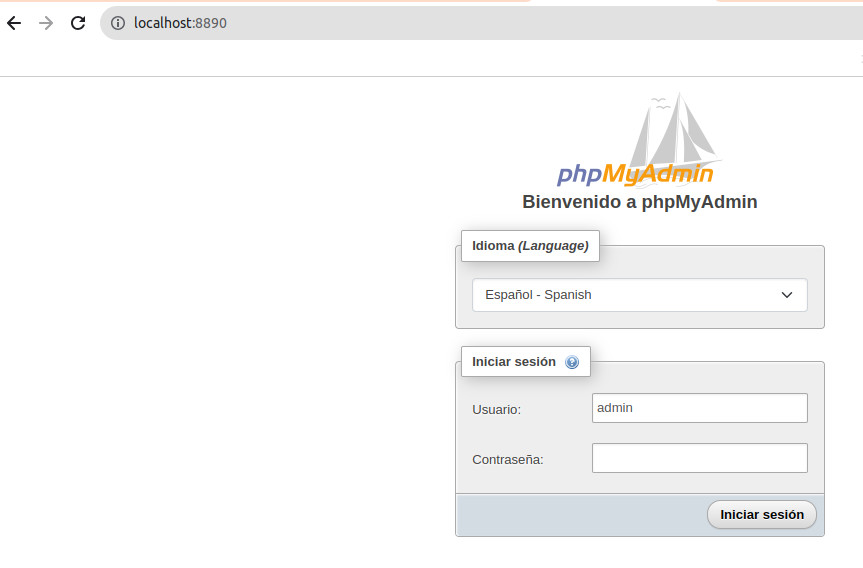
\includegraphics[scale=0.4]{images/localhost8890.jpg}
\end{center}
\caption{\label{inicio} Acceso a phpMyAdmin.}
\end{figure}
\newpage
Seleccionamos ``Importar'' en el menú superior, elegimos el archivo (\textit{database.sql} del main del proyecto) y hacemos clic en ``Importar'', situado al final de la página.
\begin{figure}[h]
\begin{center}
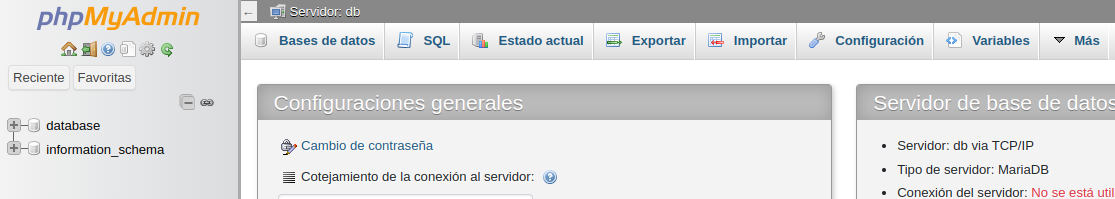
\includegraphics[scale=0.4]{images/phpMyAdmin_main.png}
\end{center}
\caption{\label{inicio} Importar en phpMyAdmin.}
\end{figure}
\begin{figure}[h]
\begin{center}
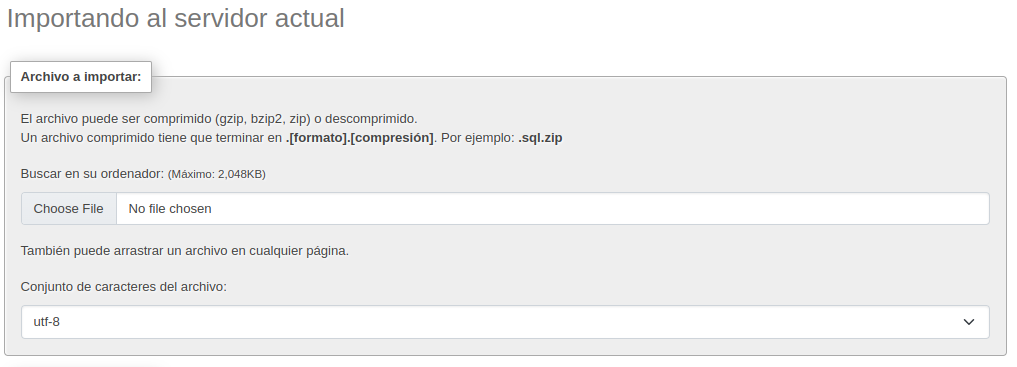
\includegraphics[scale=0.44]{images/importar_phpMyAdmin.png}
\end{center}
\caption{\label{inicio} Seleccionar base de datos.}
\end{figure}
\begin{figure}[h]
\begin{center}
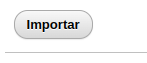
\includegraphics[scale=1]{images/botón_importar.png}
\end{center}
\caption{\label{inicio} Finalizar importación en phpMyAdmin.}
\end{figure}
\newpage
\end{comment}
Accederemos al sistema web introduciendo \hyperlink{http://localhost:81/}{http://localhost:81/} en el navegador. Nos aparecerá la página principal.\\
\newline
En ella disponemos de un menú superior con las opciones de ``Crear entrada'' y ``Login''. Con una sesión iniciada, se mostrará la opción de ``Modificar datos'' y se sustituirá el inicio de sesión por ``Logout''. Podremos ver el número de usuarios registrados en el sistema, y una tabla con los horóscopos almacenados. \\
También nos sale información sobre la cantidad de usuarios registrados en el sistema y una tabla con los horóscopos o entradas que se han introducido en el sistema, desde la que podremos ver los detalles de cada elemento, editarlo e incluso eliminarlo.\\
\begin{figure}[h]
\begin{center}
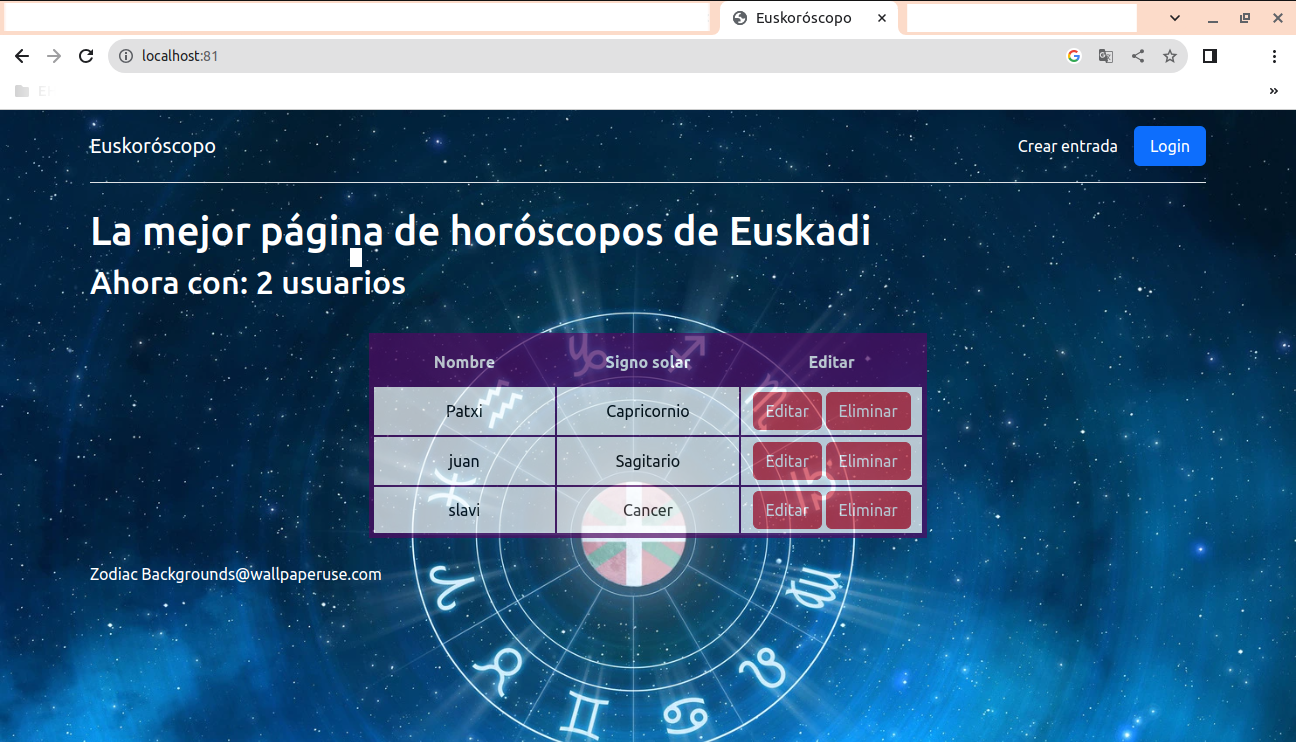
\includegraphics[scale=0.3]{images/index.png}
\end{center}
\caption{\label{inicio} Página principal.}
\end{figure}
\begin{figure}[h]
\begin{center}
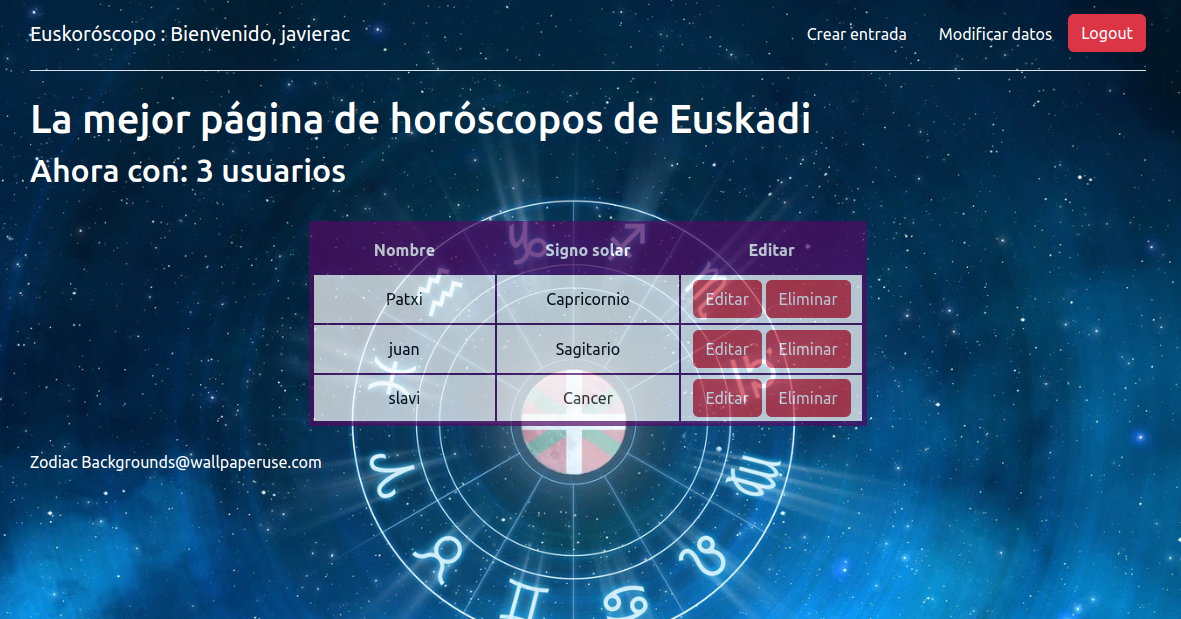
\includegraphics[scale=0.33]{images/index_logged.png}
\end{center}
\caption{\label{inicio} Página principal con sesión iniciada.}
\end{figure}
\clearpage

\section{Registro e Inicio de Sesión}
La funcionalidad tanto de registro como de identificación se ubican en la misma página, y se accede desde la página principal, pulsando sobre el botón de ``Login'' situado en la parte derecha del menú superior.
\begin{figure}[h]
\begin{center}
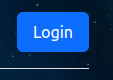
\includegraphics[scale=0.8]{images/index_login.png}
\end{center}
\caption{\label{inicio} Botón de Login.}
\end{figure}
\newline
Accederemos a ambos formularios. En el formulario superior podremos iniciar sesión, y en el inferior podremos registrarnos.
Cada uno de los campos cumple con los requisitos solicitados en el enunciado de esta primera entrega del trabajo. No los mencionaremos aquí por no ser objeto de este documento.\\
Una vez introducida la información requerida, pincharemos sobre el botón correspondiente, ``Login'' o ``Registro''.\\
Existe un usuario general para poder utilizar el sistema sin registrarse:
\begin{itemize}
    \item Usuario: \textbf{user}
    \item Contraseña: \textbf{user\\}
\end{itemize}

\begin{figure}[h]
\begin{center}
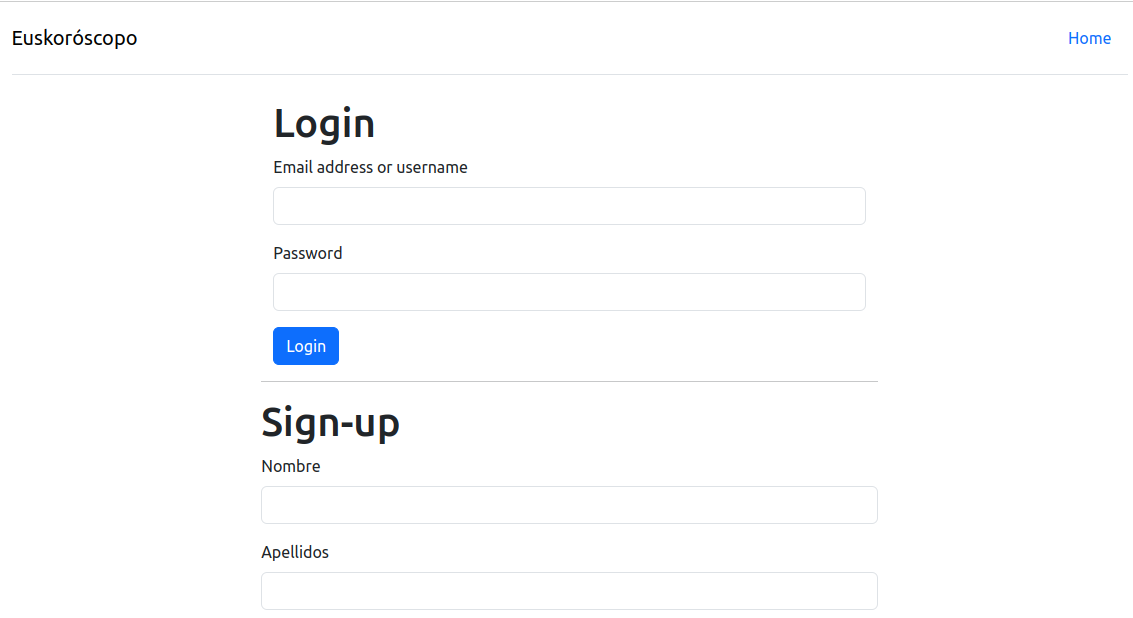
\includegraphics[scale=0.3]{images/login.png}
\end{center}
\caption{\label{inicio} Formulario de Login.}
\end{figure}
\clearpage
\begin{figure}[h]
\begin{center}
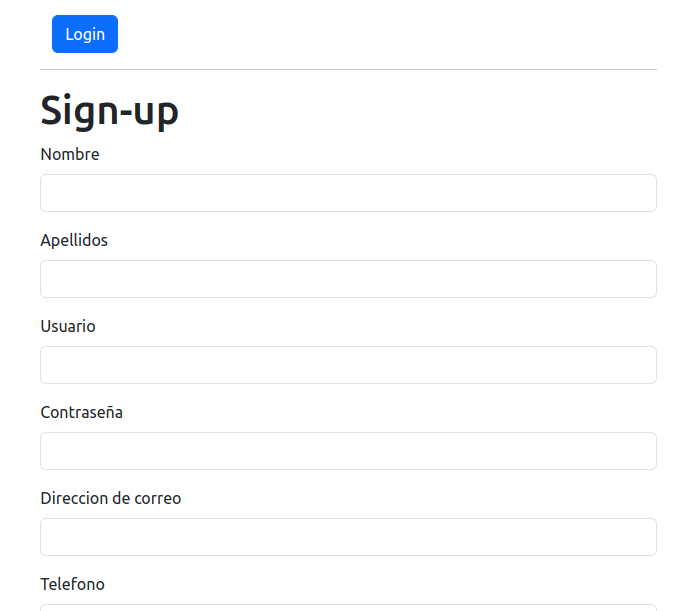
\includegraphics[scale=0.4]{images/signup.png}
\end{center}
\caption{\label{inicio} Formulario de Registro.}
\end{figure}
\begin{figure}[h]
\begin{center}
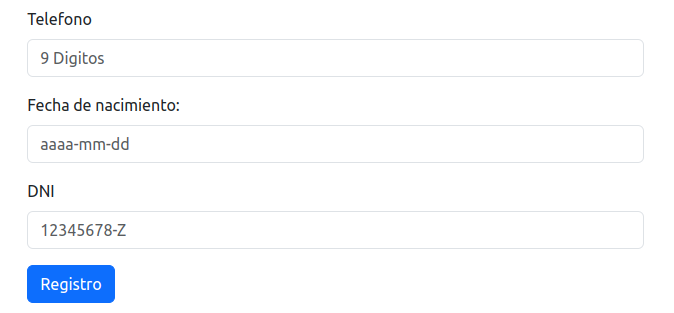
\includegraphics[scale=0.5]{images/signup2.png}
\end{center}
\caption{\label{inicio} Formulario de Registro.}
\end{figure}
\clearpage
Tanto si se introducen unos datos incorrectos de inicio de sesión como si se introduce algún dato con un formato diferente al especificado en el enunciado durante el registro, el sistema nos notificará:\\
\begin{figure}[h]
\begin{center}
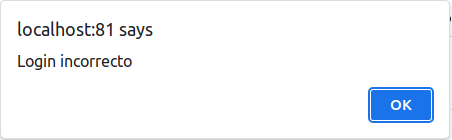
\includegraphics[scale=0.7]{images/login_error.png}
\end{center}
\caption{\label{inicio} Error inicio de sesión.}
\end{figure}
\begin{figure}[h]
\begin{center}
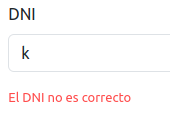
\includegraphics[scale=1]{images/signup_error.png}
\end{center}
\caption{\label{inicio} Ejemplo de error en el resgistro.}
\end{figure}
\begin{figure}[h]
\begin{center}
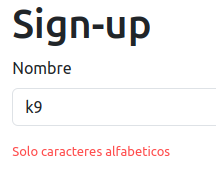
\includegraphics[scale=1]{images/signup_error2.png}
\end{center}
\caption{\label{inicio} Ejemplo de error en el resgistro.}
\end{figure}
\clearpage

\section{Modificación de datos de usuario}
Podremos modificar los datos del usuario cuya sesión está iniciada desde el menú superio.\\
Accederemos a un formulario, como el de inicio de sesión, cuyos campos han de cumplir los mismos requisitos y en los que se muestra el valor actual. Si un dato no desea modificarse, su casilla ha de dejarse en blanco.
\begin{figure}[h]
\begin{center}
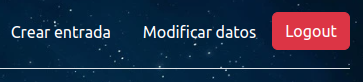
\includegraphics[scale=0.7]{images/modifyData.png}
\end{center}
\caption{\label{inicio} Botón para modificar datos de usuario.}
\end{figure}
\begin{figure}[h]
\begin{center}
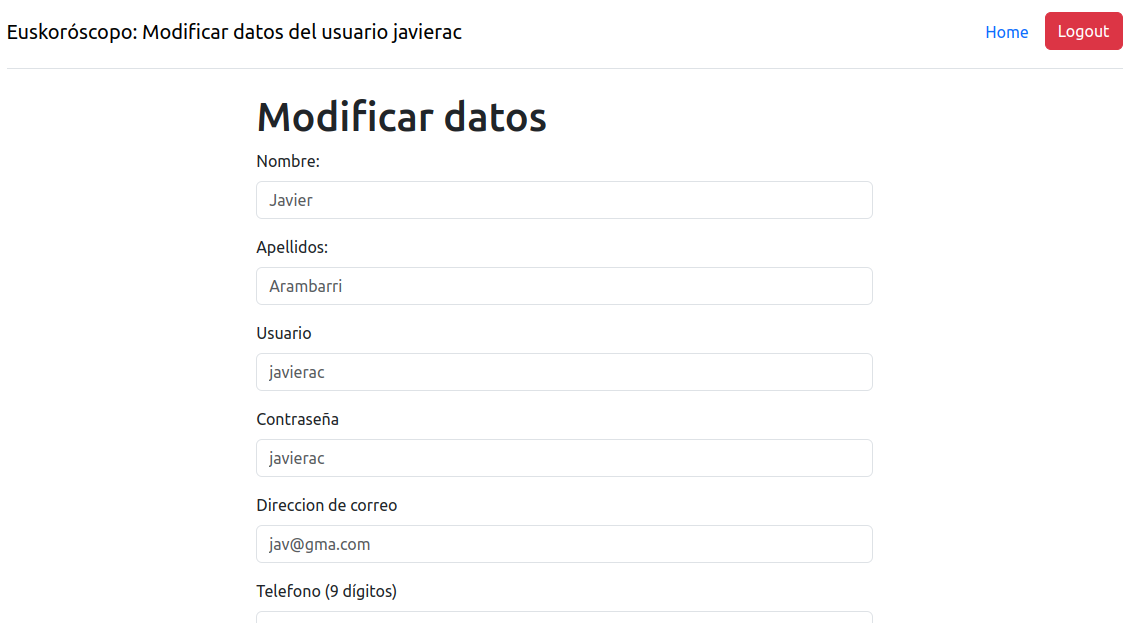
\includegraphics[scale=0.35]{images/modifyData_2.png}
\end{center}
\caption{\label{inicio} Modificar datos de usuario.}
\end{figure}
\begin{figure}[h]
\begin{center}
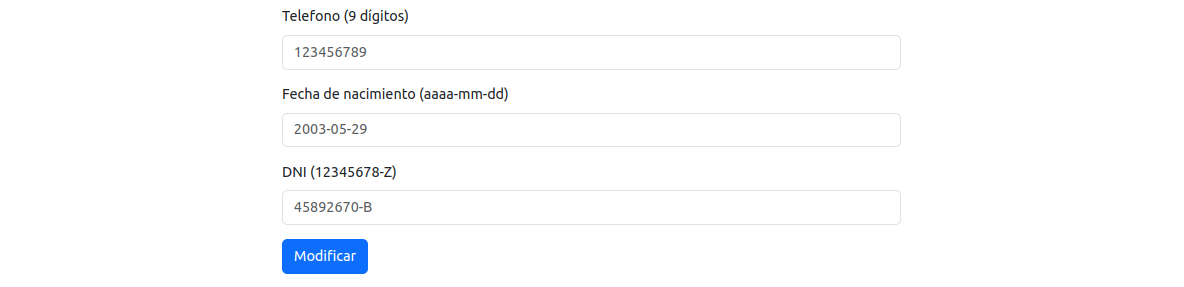
\includegraphics[scale=0.35]{images/modifyData_3.png}
\end{center}
\caption{\label{inicio} Modificar datos de usuario.}
\end{figure}
\clearpage

\section{Creación de una entrada}
Para añadir un nuevo horóscopo al sistema no será necesario estar dado de alta.
\begin{figure}[h]
\begin{center}
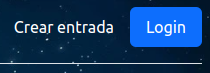
\includegraphics[scale=0.7]{images/crearEntrada.png}
\end{center}
\caption{\label{inicio} Botón para crear una nueva entrada.}
\end{figure}
\begin{figure}[h]
\begin{center}
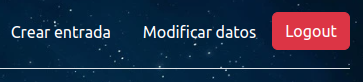
\includegraphics[scale=0.7]{images/modifyData.png}
\end{center}
\caption{\label{inicio} Botón para crear una nueva entrada.}
\end{figure}
\newline
Accedemos al formulario en el que ingresaremos los datos de la nueva entrada, y pulsamos añadir.
\begin{figure}[h]
\begin{center}
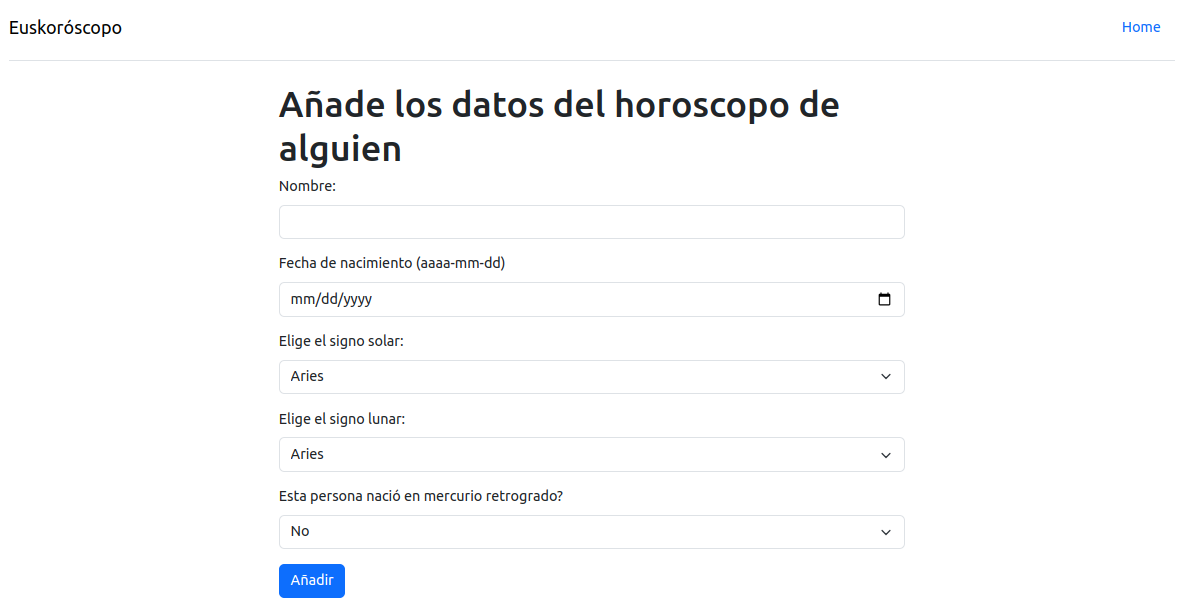
\includegraphics[scale=0.37]{images/crearEntrada2.png}
\end{center}
\caption{\label{inicio} Formulario para crear una nueva entrada.}
\end{figure}
\newline
Las nuevas entradas se mostrarán en la tabla de la página principal.
\clearpage

\section{Edición de una entrada}
Para editar una entrada existente lo haremos desde la página principal. En la tabla de los horóscopos pincharemos el botón de editar de la entrada que deseamos modificar.\\
Accederemos al formulario de edición, que funciona de la misma manera que el de modificación de los datos del usuario registrado. Pulsaremos el botón ``Modificar'' y se actualizan los campos que se han rellenado.
\begin{figure}[h]
\begin{center}
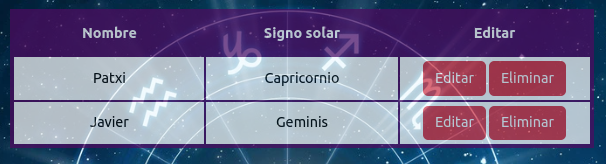
\includegraphics[scale=0.65]{images/editarEntrada.png}
\end{center}
\caption{\label{inicio} Editar una entrada.}
\end{figure}
\begin{figure}[h]
\begin{center}
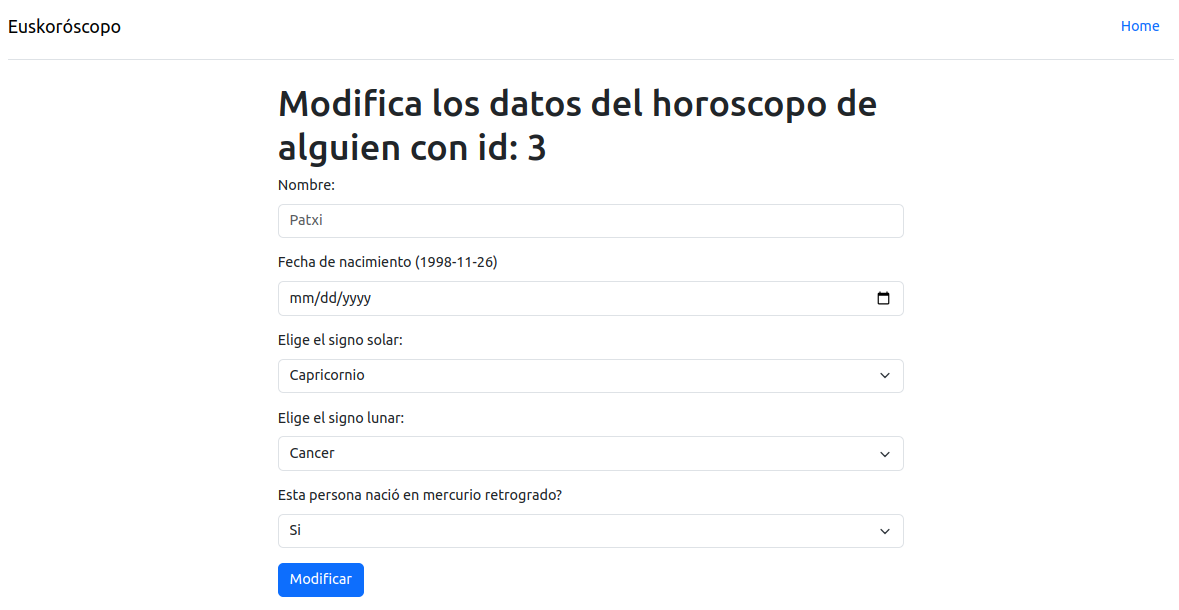
\includegraphics[scale=0.37]{images/editarEntrada2.png}
\end{center}
\caption{\label{inicio} Formulario para editar una entrada.}
\end{figure}
\clearpage

\section{Eliminación de una entrada}
Las entradas se eliminarán de la misma manera en que se editan, pero pulsando el botón ``Eliminar'' desde la página principal. Una vez eliminada, nos indicará que se ha realizado correctamente la actualización en el sistema.
\begin{figure}[h]
\begin{center}
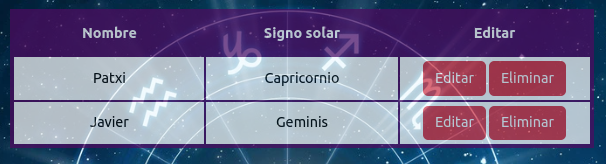
\includegraphics[scale=0.65]{images/editarEntrada.png}
\end{center}
\caption{\label{inicio} Editar una entrada.}
\end{figure}
\begin{figure}[h]
\begin{center}
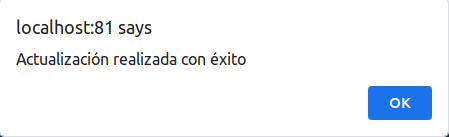
\includegraphics[scale=0.65]{images/actualización.png}
\end{center}
\caption{\label{inicio} Mensaje de confimación.}
\end{figure}
\clearpage

\section{Mensajes de actualización}
Cada vez que se actualice algún dato o se interactúe con el funcionamiento del sistema, ya sea al modificar los datos de usuario y entradas, iniciar sesión, eliminar entrada o... se mostrarán mensajes de alerta indicándolo.\\
\begin{figure}[h]
\begin{center}
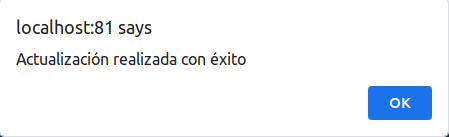
\includegraphics[scale=0.7]{images/actualización.png}
\end{center}
\caption{\label{inicio} Alerta ``actualización exitosa''.}
\end{figure}
\begin{figure}[h]
\begin{center}
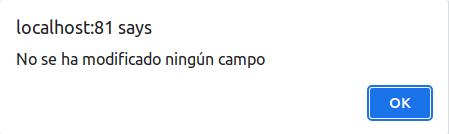
\includegraphics[scale=0.7]{images/actualización2.png}
\end{center}
\caption{\label{inicio} Alerta ``no se ha modificado ningún campo''.}
\end{figure}
\begin{figure}[h]
\begin{center}
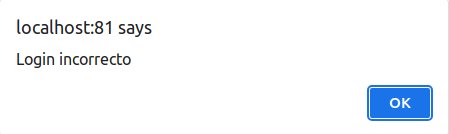
\includegraphics[scale=0.7]{images/actualización3.png}
\end{center}
\caption{\label{inicio} Alerta ``Login incorrecto''.}
\end{figure}
\begin{figure}[h]
\begin{center}
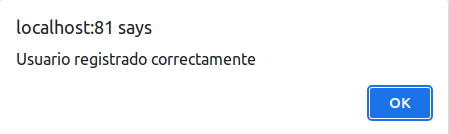
\includegraphics[scale=0.7]{images/actualización4.png}
\end{center}
\caption{\label{inicio} Alerta ``Usuario registrado correctamente''.}
\end{figure}
\begin{figure}[h]
\begin{center}
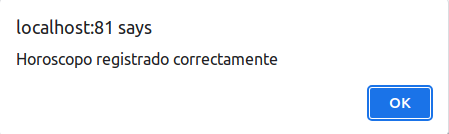
\includegraphics[scale=0.7]{images/actualización5.png}
\end{center}
\caption{\label{inicio} Alerta ``Horóscopo registrado correctamente''.}
\end{figure}


\end{document}